%%%%%%%%%%%%%%%%%%%%%%%%%%%%%%%%%%%%%%%%%
% Beamer Presentation
% LaTeX Template
% Version 1.0 (10/11/12)
%
% This template has been downloaded from:
% http://www.LaTeXTemplates.com
%
% License:
% CC BY-NC-SA 3.0 (http://creativecommons.org/licenses/by-nc-sa/3.0/)
%
%%%%%%%%%%%%%%%%%%%%%%%%%%%%%%%%%%%%%%%%%

%-------------------------------------------------------------------------------
%	PACKAGES AND THEMES
%-------------------------------------------------------------------------------

\documentclass{beamer}
\usepackage{xcolor}
\usepackage{graphicx}
\usepackage{tikz}
\usepackage{listings}
\usepackage{multicol}

\DeclareMathOperator{\diag}{diag}

\definecolor{applegreen}{rgb}{0.55, 0.71, 0.0}
\definecolor{blue(ncs)}{rgb}{0.0, 0.45, 0.60}
\definecolor{burgundy}{rgb}{0.5, 0.0, 0.13}

\definecolor{cadet}{rgb}{0.33, 0.41, 0.47}
\definecolor{airforceblue}{rgb}{0.36, 0.54, 0.66}

\mode<presentation> {

\usetheme{CambridgeUS}

\usecolortheme{wolverine}

\definecolor{gold}{HTML}{D4A017}
\definecolor{darkgold}{HTML}{B7950B}

\setbeamercolor{palette primary}{bg=cadet,fg=white}
\setbeamercolor{palette secondary}{bg=airforceblue,fg=white}
\setbeamercolor{palette tertiary}{bg=black,fg=white}
\setbeamercolor{palette quaternary}{bg=cadet,fg=white}

\setbeamercolor{frametitle}{bg=airforceblue,fg=white}

\setbeamercolor{section number projected}{bg=black,fg=cadet}
\setbeamercolor{item}{fg=black,bg=cadet}

\setbeamertemplate{page number in head/foot}[framenumber]

\lstset{basicstyle=\ttfamily\footnotesize,breaklines=true}
}



\lstdefinestyle{colouredC}{ 
  commentstyle=\color[gray]{0.4},
  keywordstyle=\bfseries,
  keywordstyle=[2]\color[rgb]{0.75, 0, 0},
  keywordstyle=[3]\color[rgb]{0, 0.5, 0},
  keywordstyle=[4]\color[rgb]{0, 0.5, 0},
  keywordstyle=[5]\color[rgb]{0, 0, 0.75},
  numberstyle=\tiny\color{mGray},
  stringstyle=\color[rgb]{0, 0, 0.5},
  basicstyle=\ttfamily,
  language=C,
  morekeywords=[3]{CeedInt, CeedScalar},
}

\lstdefinestyle{boxedC}{
  style=colouredC,
  numbers=left,
  firstnumber=auto,
  numberblanklines=true,
  frame=trbL,
  numberstyle=\tiny,
  frame=leftline,
  numbersep=7pt,
  framesep=5pt,
  framerule=10pt,
  xleftmargin=15pt,
  backgroundcolor=\color[gray]{0.97},
  rulecolor=\color[gray]{0.90}%
}

\usepackage{graphicx} % Allows including images
\usepackage{booktabs} % Allows the use of \toprule, \midrule and \bottomrule in tables

%----------------------------------------------------------------------------------------
%	TITLE PAGE
%----------------------------------------------------------------------------------------

\title[UO AMD APU Workshop]{University of Oregon\\AMD APU Workshop
} % The short title appears at the bottom of every slide, the full title is only on the title page

\author{Jeremy L Thompson} % Your name
\institute[CU Boulder] % Your institution as it will appear on the bottom of every slide, may be shorthand to save space
{University of Colorado Boulder \\ % Your institution for the title page
\medskip
\textit{jeremy@jeremylt.org} % Your email addressintention
}
\date{13 Feb 2025} % Date, can be changed to a custom date

\begin{document}

\begin{frame}
\titlepage % Print the title page as the first slide
\end{frame}

%------------------------------------------------

\begin{frame}
\frametitle{Overview} % Table of contents slide, comment this block out to remove it
\tableofcontents % Throughout your presentation, if you choose to use \section{} and \subsection{} commands, these will automatically be printed on this slide as an overview of your presentation
\end{frame}

%------------------------------------------------
\section{Introduction}
%------------------------------------------------

\begin{frame}
\frametitle{libCEED, Ratel, and HONEE Team}

\begin{center}
\includegraphics[height=2.75cm]{libCEEDlogo.png}
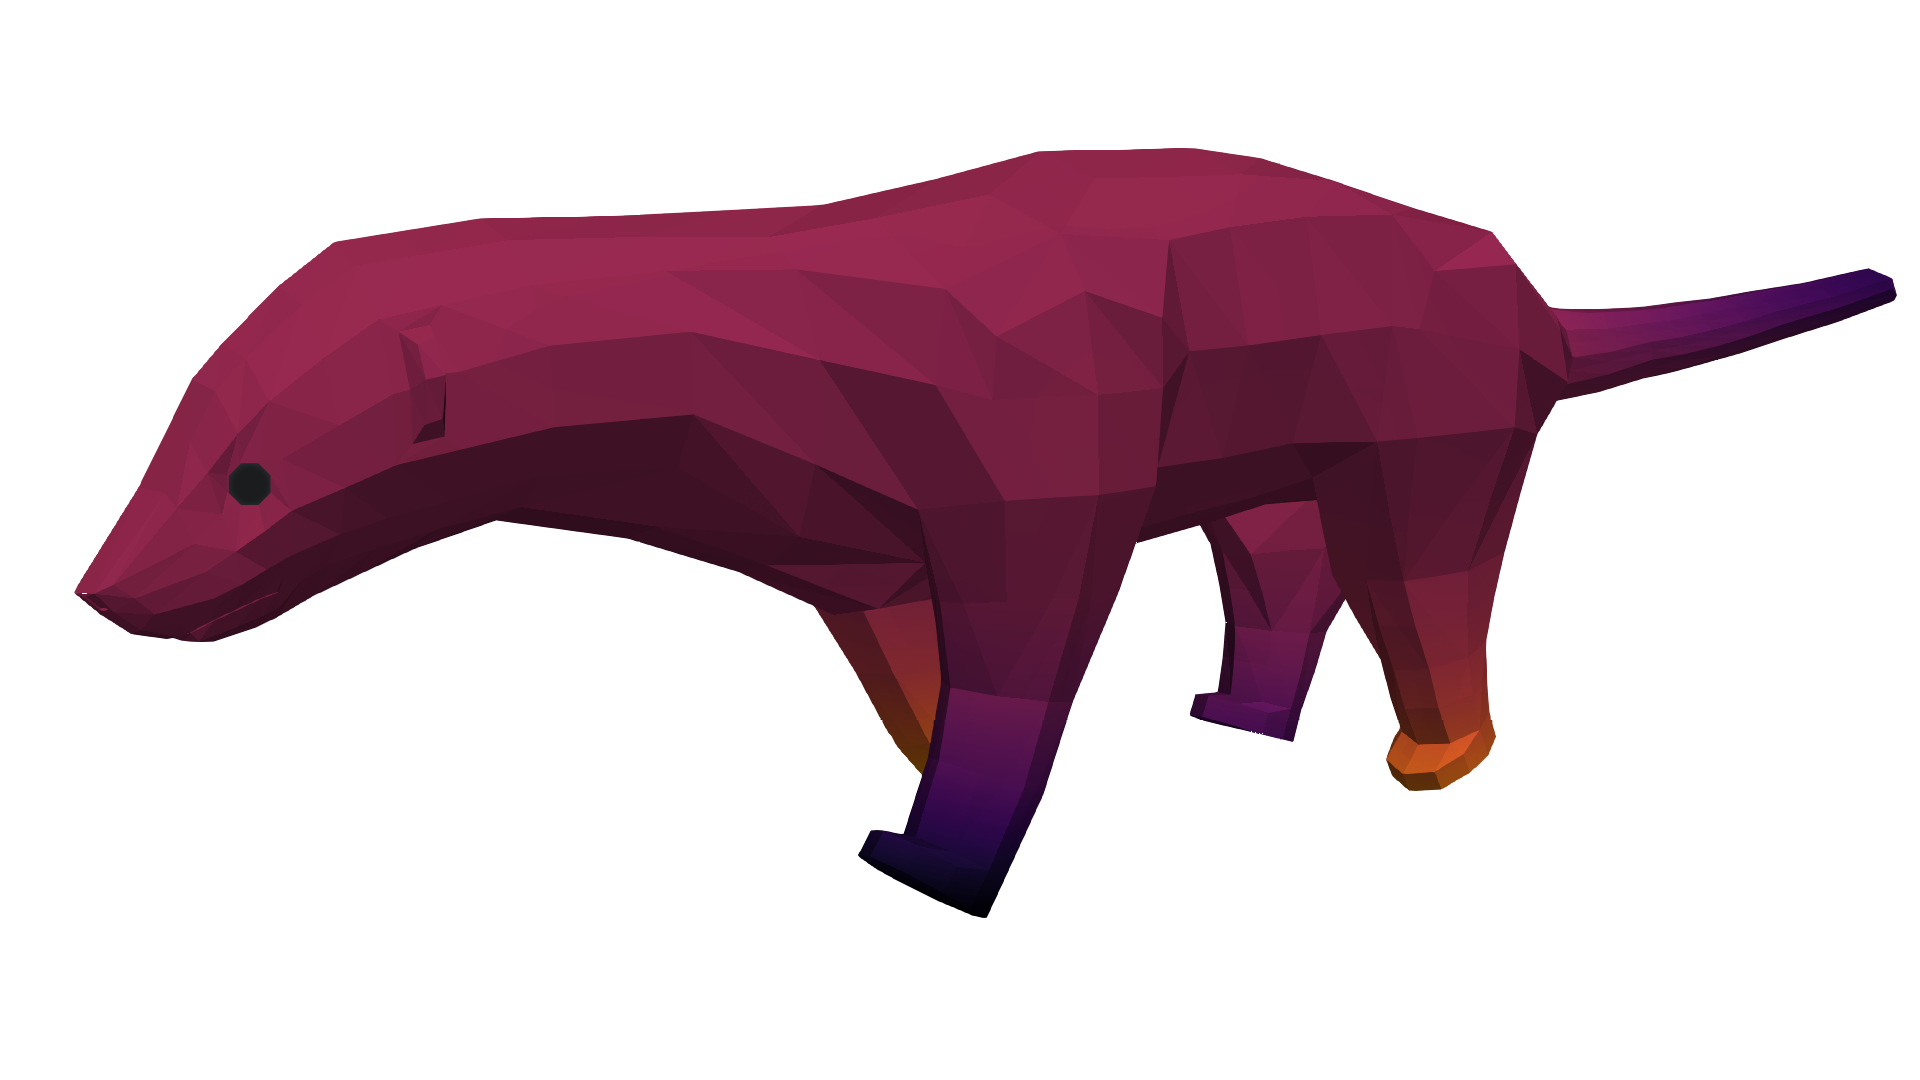
\includegraphics[height=2.75cm]{Ratellogo.png}
\end{center}

{\flushleft

libCEED Repo: https://github.com/CEED/libCEED\\
HONEE Repo: https://gitlab.com/phypid/HONEE\\
Ratel Repo: https://gitlab.com/micromorph/ratel\\

~\\
Developers: \textbf{Zach Atkins}, Jed Brown, Fabio Di Gioacchino, Leila Ghaffari,\\
\hspace{19mm} Kenneth Jansen, \textbf{Rezgar Shakeri}, James Wright,\\
\hspace{19mm} \textbf{Jeremy L Thompson}\\

~\\

{\tiny The authors acknowledge support by the Department of Energy, National Nuclear Security Administration, Predictive Science\\Academic Alliance Program (PSAAP) under Award Number DE-NA0003962.}

}

\begin{center}

\includegraphics[height=0.7cm]{psaap-center-logos}
\end{center}

\end{frame}

%------------------------------------------------

\begin{frame}
\begin{center}
\frametitle{Matrix-Free Operators from libCEED}

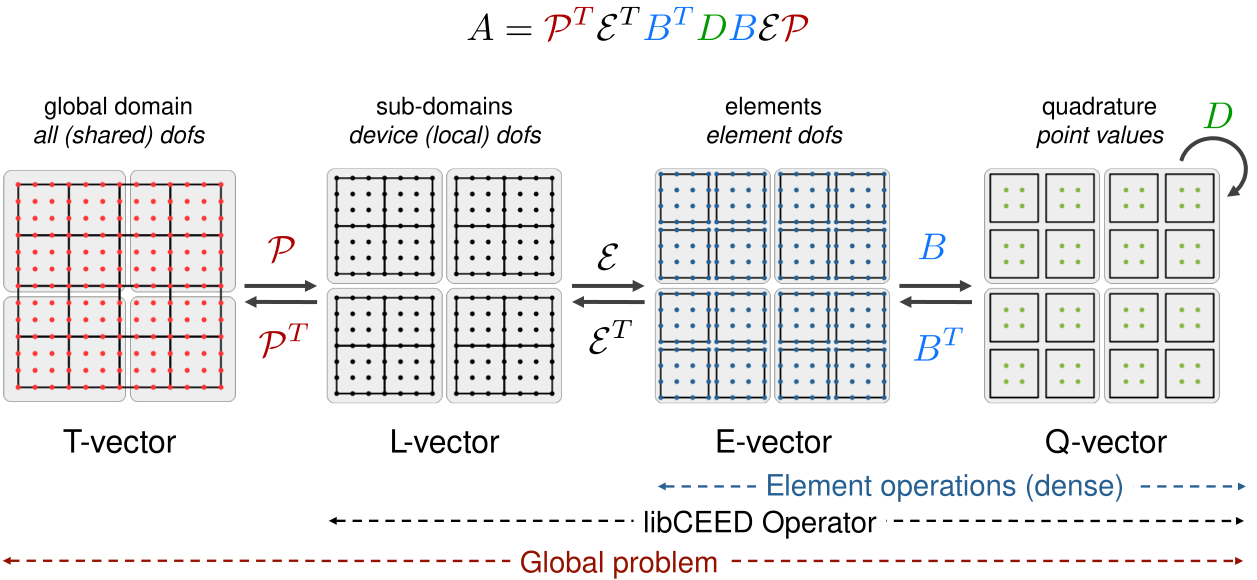
\includegraphics[height=5.0cm]{libCEEDAPI.png}

~\\

libCEED provides arbitrary order matrix-free operator evaluation\\

\end{center}
\end{frame}

%------------------------------------------------

\begin{frame}
\begin{center}
\frametitle{Workshop Goals}

\begin{itemize}

\item CPU/GPU unified memory space testing and optimization\\

~\\

\item Basis kernel optimization, standard and AtPoints quadrature\\

~\\

\item Better understand user QF performance and best practices\\

~\\

\item Diagonal and full assembly kernel tuning\\

\end{itemize}

\end{center}
\end{frame}

%------------------------------------------------
\section{Day 2}
%------------------------------------------------

\begin{frame}
\begin{center}
\frametitle{Day 2 Update}

\begin{itemize}

\item libCEED and PETSc built on Odyssey\\

~\\

\item Basic profiling runs of Bakeoff Problems\\

~\\

\begin{itemize}

\item \lstinline{rocprof-sys} providing time in each kernel\\

~\\

\item Using \lstinline{/gpu/hip/shared} over \lstinline{/gpu/hip/gen} shows clearer picture\\

~\\

\item Goal is to create full flame graphs with CPU call stack\\

~\\

\item Have identified hand-rolled kernels to be replaced with HIP utils\\

\end{itemize}

~\\

\item As expected - user QFunction kernels are bulk of time\\

~\\

\begin{itemize}

\item How can we ID performance issues for single kernel?\\

~\\

\item Hope to generate "best practices" guide for users\\

\end{itemize}

~\\

\end{itemize}

\end{center}
\end{frame}

%------------------------------------------------

\begin{frame}[fragile]
\begin{center}
\frametitle{Sample Flamegraph}

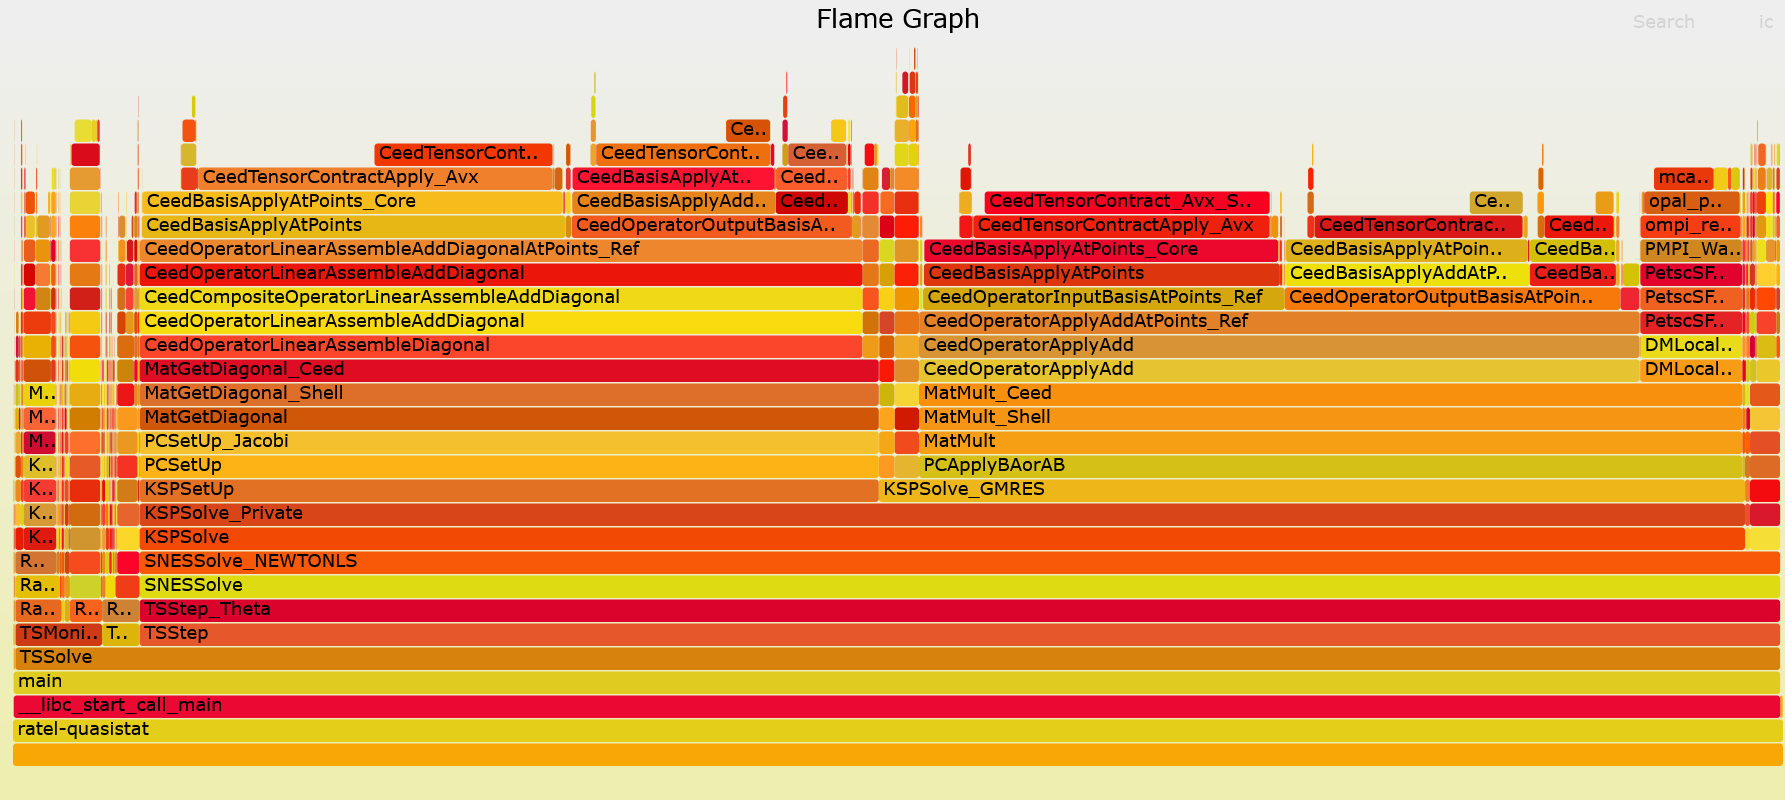
\includegraphics[height=5.0cm]{CPUFlamegraph.png}

Currently getting kernel names without above CPU call stack\\

~\\

Sample \lstinline{rocprof-sys} commands:\\

{\tiny
\begin{lstlisting}[style=boxedC]
rocprof-sys-instrument -o ex2.inst -- ./build/ex2-surface
rocprof-sys-run -- ./ex2.inst -c /gpu/hip/shared -b 20000 -s 5000000
\end{lstlisting}
}

\end{center}
\end{frame}

%------------------------------------------------
\section{Day 3}
%------------------------------------------------

\begin{frame}
\begin{center}
\frametitle{Day 3 Update}

\begin{itemize}

\item libCEED and Ratel performance exploration on Odyssey\\

~\\

\item Improved profiling runs of Bakeoff Problems\\

~\\

\begin{itemize}

\item \lstinline{rocprof-sys-sample} providing full flame graphs\\

~\\

\item Using \lstinline{rocprof-sys-sample -PTDH -I all --verbose 1 --freq 50 -- ...}\\

~\\

\item High number of people on the machine providing muddy perf data\\

\end{itemize}

~\\

\item Replacing some hand-rolled replicas of BLAS operations\\

~\\

\begin{itemize}

\item Pre ROCm 6.0/CUDA 12.0 lacks \lstinline{*blas*_64} BLAS functions\\

\end{itemize}

~\\

\item Unified memory changes running, showing good improvement\\

\end{itemize}

\end{center}
\end{frame}

%------------------------------------------------
\section{Final Outbrief}
%------------------------------------------------

\begin{frame}
\begin{center}
\frametitle{Final Outbrief}

\begin{itemize}

\item Unified memory improves performance on APU hardware\\

~\\

\begin{itemize}

\item Approximately 5\% speedup with unified memory\\

\end{itemize}

~\\

\item IDed and fixed minor internal performance issues\\

~\\

\begin{itemize}

\item Prefer *BLAS calls over hand-rolled kernels where able\\

~\\

\item Prefer \lstinline{*memset()} over hand-rolled kernels when zeroing\\

~\\

\item Reduce independent memory zeroing kernel calls in \lstinline{/gpu/*/shared}\\

\end{itemize}

~\\

\item Identified tools/processes for future profiling work\\

~\\

\begin{itemize}

\item \lstinline{rocprof-sys-sample} providing flame graphs\\

~\\

\item Analyzing individual QFunctions to improve, build guidelines\\

\end{itemize}

\end{itemize}

\end{center}
\end{frame}

%------------------------------------------------
\section{Questions}
%------------------------------------------------

\begin{frame}
\frametitle{Questions?}

\begin{center}
\includegraphics[height=2.75cm]{libCEEDlogo.png}
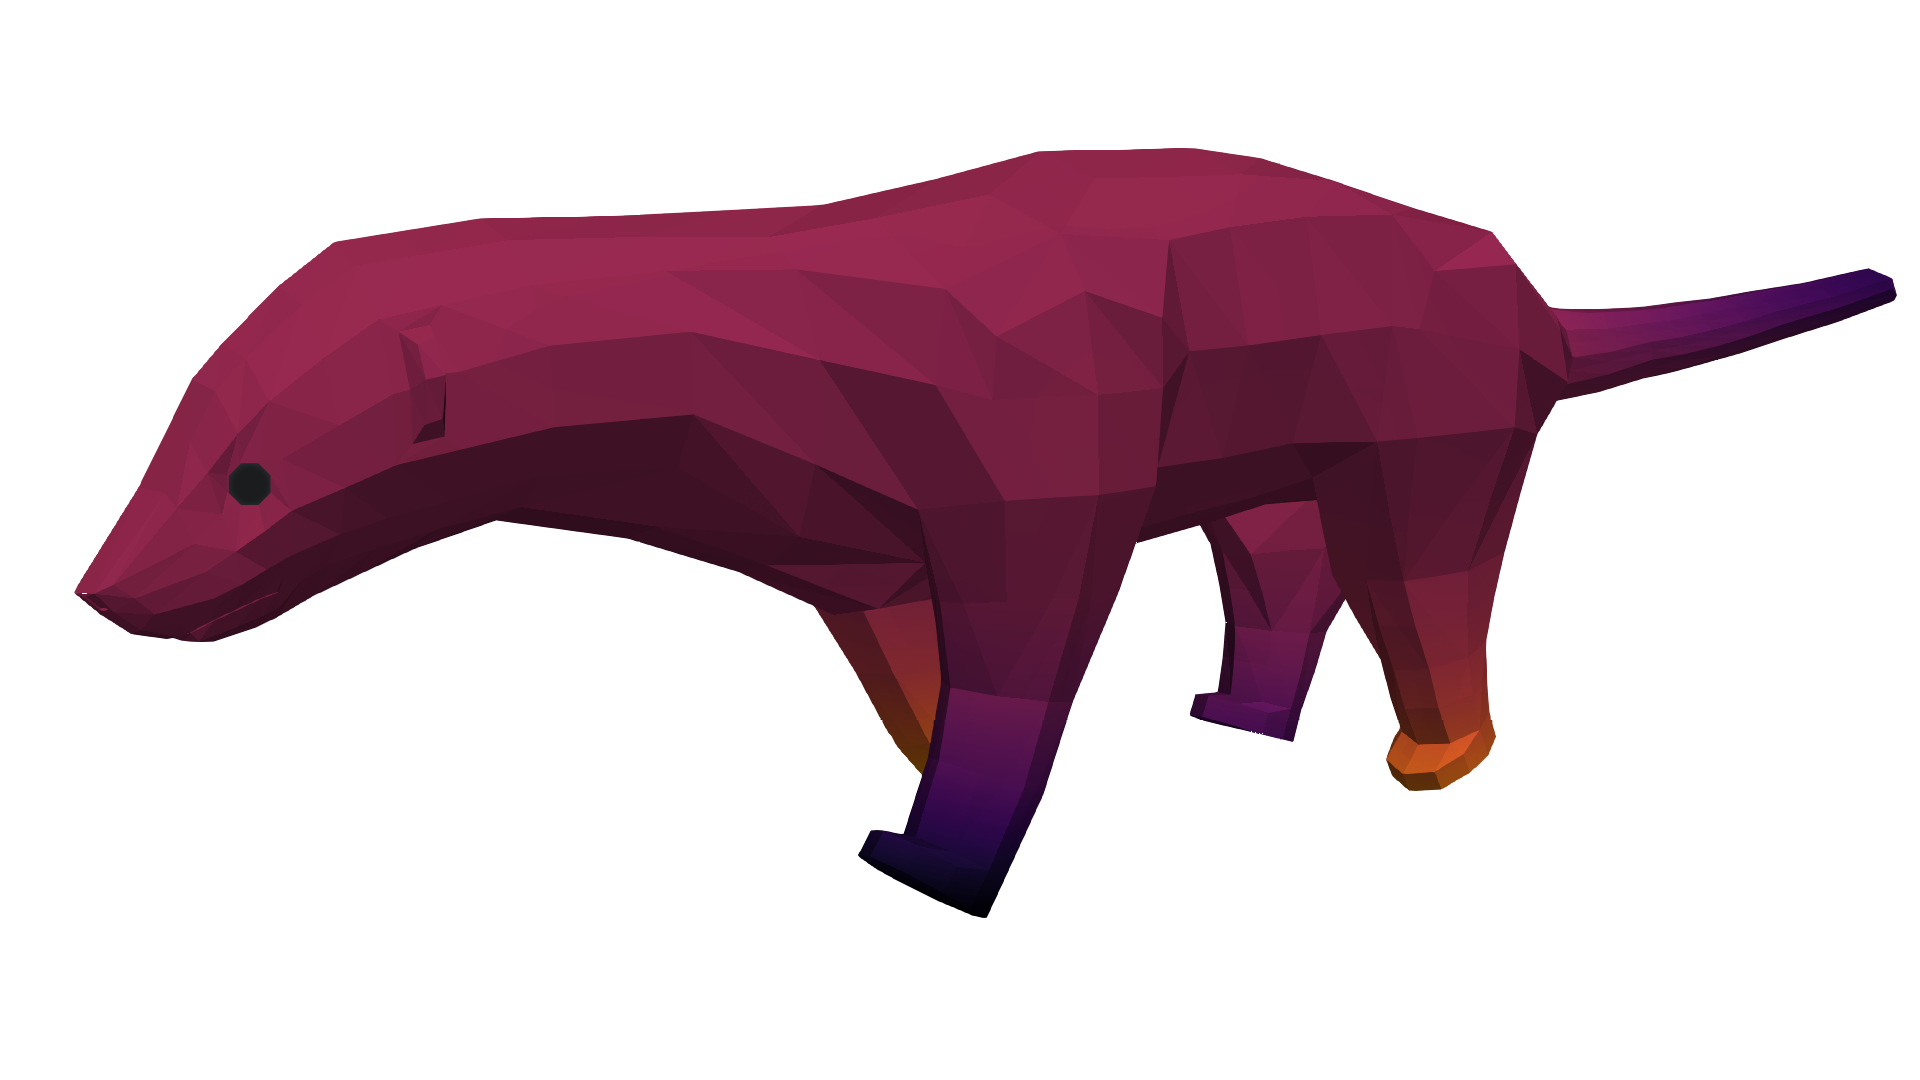
\includegraphics[height=2.75cm]{Ratellogo.png}
\end{center}

{\flushleft

libCEED Repo: https://github.com/CEED/libCEED\\
HONEE Repo: https://gitlab.com/phypid/HONEE\\
Ratel Repo: https://gitlab.com/micromorph/ratel\\

~\\

Grant: Predictive Science Academic Alliance Program (DE-NA0003962)\\

}

\begin{center}

\includegraphics[height=0.8cm]{psaap-center-logos}
\end{center}

\end{frame}

%-------------------------------------------------------------------------------

\end{document}

%-------------------------------------------------------------------------------
